\chapter {Interfacing Passive Infrared Sensor-PIR}
\thispagestyle{empty}
\label{ldr}

\newcommand{\LocLDRfig}{\Origin/user-code/pir/figures}
\newcommand{\LocLDRardcode}{\Origin/user-code/pir/arduino}
\newcommand{\LocLDRardbrief}[1]{{\tt
      \seqsplit{Origin/user-code/pir/arduino/#1}},
  see \fnrefp{fn:file-loc}}

%%%%%%%%%python
\newcommand{\LocLDRpycode}{\Origin/user-code/pir/python}
\newcommand{\LocLDRpybrief}[1]{{\tt \seqsplit{%
        Origin/user-code/pir/python/#1}}, see \fnrefp{fn:file-loc}}
%%%%%%python



The PIR sensor is responsible for detecting the change in infrared radiation levels when an intruder or human is passed through the system or space where it is arranged. Depending on the change in radiation levels the change in voltages occurs and then with this voltage the signal is amplified and hence the sound will be produced. Thus, it is helpful in various applications and areas. This type of system has many advantages compared to the existing system. 

When motion is detected, it is displayed on the screen and in the next phase of this project, when motion is detected, it is displayed in an LCD. 

\section{Preliminary}
This system can be broadly divided into 2 small parts namely:  Motion detection using PIR sensor, Motion detection using PIR sensor and displaying on LCD.
\begin{itemize}
  \item \textbf{Motion detection using PIR sensor}: - In this part a PIR sensor is used to detect motion. PIR becomes HIGH (gives output 1) when motion is detected and becomes LOW when no motion is detected or when the motion ends.
So in this part using Arduino and python, we will receive output “No Motion” initially until any motion is detected. The output “Motion detected!” will be displayed when we the sensor encounters motion and the output “Motion ended!” will be displayed when the motion ends. The Ground pin of PIR sensor is connected to GND of Arduino, The VCC of PIR sensor is connected to 5V and the data pin is connected to digital pin 6 of Arduino.

  \item \textbf{Motion detection using PIR sensor and displaying on LCD}: - In this part PIR and LCD is used. Working is same as previous part. But the output will be displayed in the LCD than in the monitor. The connections of PIR is same as previous part. 
\end{itemize}
\begin{figure}[hpt]
  \centering
    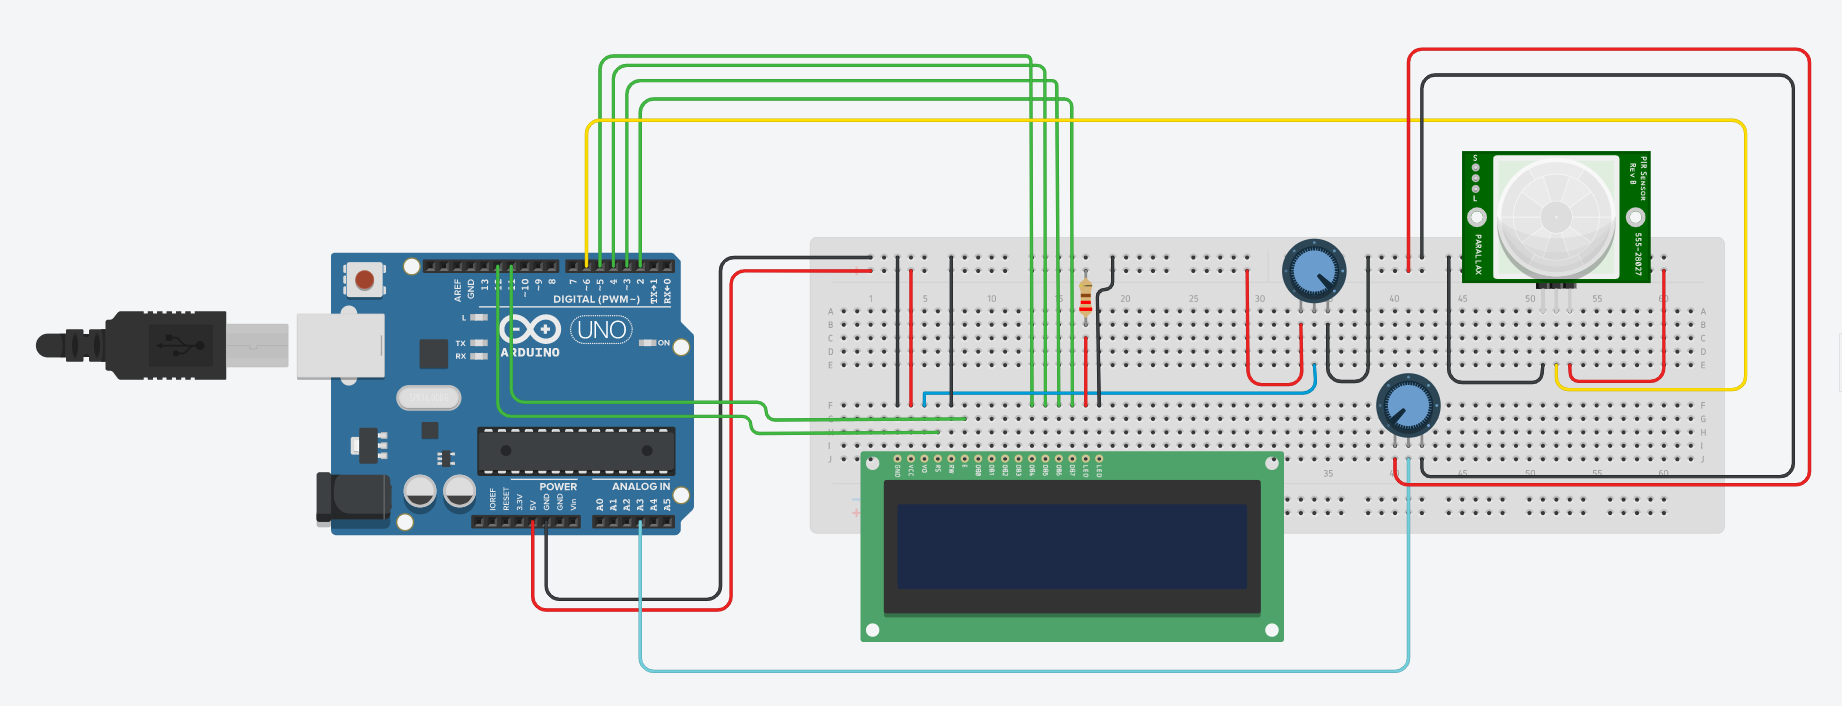
\includegraphics[width=\textwidth]{\LocLDRfig/propsys.png}
    \label{fig:propsys} \hfill
  \caption{Proposed system for motion detection for PIR Interfacing}
\end{figure} 

\section{PIR Sensor HC-SR501}
A passive infrared sensor is an electronic sensor that measures infrared light radiating from objects. PIR sensors mostly used in PIR-based motion detectors.
PIR sensor is specially designed to detect such levels of infrared radiation. It basically consists of two main parts: A Pyroelectric Sensor and A special lens called Fresnel lens which focuses the infrared signals onto the pyroelectric sensor.
A Pyroelectric Sensor actually has two rectangular slots in it made of a material that allows the infrared radiation to pass. Behind these, are two separate infrared sensor electrodes, one responsible for producing a positive output and the other a negative output. The reason for that is that we are looking for a change in IR levels and not ambient IR levels. The two electrodes are wired up so that they cancel each other out. If one half sees more or less IR radiation than the other, the output will swing high or low.


\begin{figure}[hpt]
  \centering
    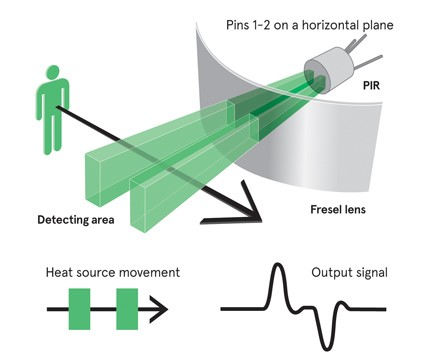
\includegraphics[width=\textwidth]{\LocLDRfig/pyrosensor.jpg}
    \label{fig:pyro} \hfill
  \caption{Pyroelectric Sensor}
\end{figure}


When the sensor is idle, i.e. there is no movement around the sensor; both slots detect the same amount of infrared radiation, resulting in a zero output signal.
But when a warm body like a human or animal passes by; it first intercepts one half of the PIR sensor, which causes a positive differential change between the two halves. When the warm body leaves the sensing area, the reverse happens, whereby the sensor generates a negative differential change. The corresponding pulse of signals results in the sensor setting its output pin high.

There are two potentiometers on the board to adjust a couple of parameters:
\begin{itemize}
  \item \textbf{Sensitivity}– This sets the maximum distance that motion can be detected. It ranges from 3 meters to approximately 7 meters. The topology of your room can affect the actual range you achieve.
  \item \textbf{Time}– This sets how long that the output will remain HIGH after detection. At minimum it is 3 seconds, at maximum it is 300 seconds or 5 minutes.
\end{itemize}
 
It has two settings:
\begin{itemize}
  \item 	H– This is the Hold/Repeat/Retriggering. In this position the HC-SR501 will continue to output a HIGH signal as long as it continues to detect   movement.
  \item  L– This is the Intermittent or No-Repeat/Non- Retriggering In this position the output will stay HIGH for the period set by the TIME potentiometer adjustment.
\begin{figure}[hpt]
  \centering
  \subfloat[No-Repeat/Non- Retriggering  charactiristics]{
    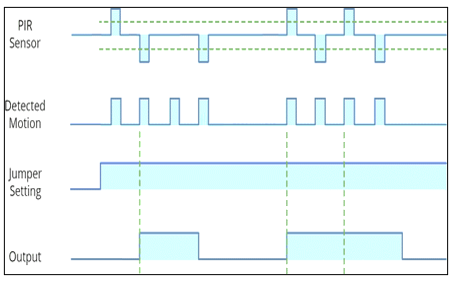
\includegraphics[width=\smfig]{\LocLDRfig/h.png}
    \label{fig:h}} \hfill
  \subfloat[Symbolic representation of an LDR]{
    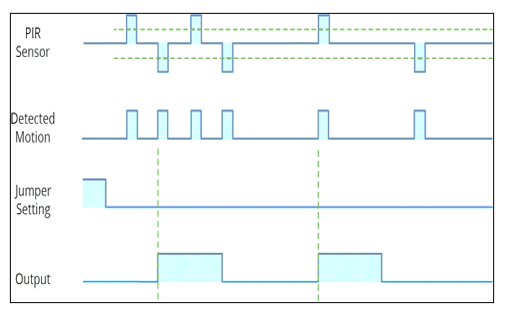
\includegraphics[width=\smfig]{\LocLDRfig/l.png}
    \label{fig:l}}
  \caption{Settings of PIR Sensor}
\end{figure}
\end{itemize}
\begin{figure}[hpt]
  \centering
    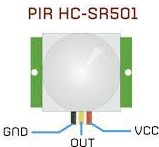
\includegraphics[width=\smfig]{\LocLDRfig/pirpinout.jpg}
    \label{fig:pinp} \hfill
  \caption{Pinout of PIR sensor}
\end{figure} 
\subsection{PIR sensor PINOUT}


\begin{itemize}
  \item \textbf{VCC} is the power supply for HC-SR501 PIR sensor which we connect the 5V pin on the Arduino.
  \item \textbf{Output} pin is a 3.3V TTL logic output. LOW indicates no motion is detected, HIGH means some motion has been detected.
  \item \textbf{GND} should be connected to the ground of Arduino.
\end{itemize}

\section{Interfacing the PIR through the Arduino IDE}
\label{sec:pir-arduino-code}
\subsection{Interfacing the PIR}
In this section, we shall describe how to read the voltage values from a HC-SR501 PIR Sensor connected to the digital pin 6 of the Arduino Uno board. The HC-SR501 PIR Sensor has to be connected to the Arduino Uno board before doing these experiments and the Arduino Uno needs to be connected to the computer with a USB cable, as shown in \figref{fig:propsys}.

\begin{enumerate}
  \item Read the digital value of PIR sensor as mentioned above using digitalRead function.
        \lstinputlisting[firstline=12,lastline=12]
        {\LocLDRardcode/pir/pir.ino}
\item The value received by digitalRead will be 0/1 (HIGH/LOW) depending upon whether motion is detected or not detected by PIR sensor. The received value is printed in serial monitor.
        \lstinputlisting[firstline=17,lastline=17]
        {\LocLDRardcode/pir/pir.ino}
\item Delay is added to slow down the rate of output being printed in serial monitor.
        \lstinputlisting[firstline=19,lastline=19]
        {\LocLDRardcode/pir/pir.ino}
The functions are written inside void loop and the operations will keep on working till the Arduino code executes.    

\end{enumerate}


\subsection{Arduino Code}
\label{sec:ldr-arduino-code}
\addtocontents{ard}{\protect\addvspace{\codclr}}

\begin{ardcode}
  \acaption{Read and display the PIR values}
  {Read and display the PIR values.  Available at
    \LocLDRardbrief{ldr-read/led-read.ino}.}
  \label{ard:ldr-read}
  \lstinputlisting{\LocLDRardcode/pir/pir.ino}
\end{ardcode}





\section{Interfacing the PIR through Python}
\subsection{Interfacing the PIR}
In this section, we discuss how to carry out the experiments of the section \secref{sec:pir-arduino-code} using Python. We will list the same experiment. The HC-SR501 should be attached to the Arduino Uno board before doing these experiments and the Arduino Uno needs to be connected to the computer with a USB cable, as shown in \figref{fig:propsys} .The Firmware code given in appendix should be uploaded to the Arduino board. 

\begin{enumerate}
  \item Declare the pin used for the HC-SR501 using a variable and creating a counter variable. 
        \lstinputlisting[firstline=23,lastline=25]
        {\LocLDRpycode/PIR-FOSSEE.py} 
 \item The Python command used for digitalRead function is, 
        \lstinputlisting[firstline=27,lastline=27]
        {\LocLDRpycode/PIR-FOSSEE.py} 
 \item The output Motion detected, Motion ended and No Motion are printed based on the input received      from PIR sensor and the pirstate variable. Initially pirstate is 0, and until the input from the Sensor is 1(High), the output printed in python screen will be “No Motion”. Once the Sensor detects motion(give input 1), pirstate is changed to 1 and the output “Motion detected” is printed. Then once the input becomes 0(LOW), the output printed on python screen will be “Motion Ended”.
        \lstinputlisting[firstline=29,lastline=37]
        {\LocLDRpycode/PIR-FOSSEE.py} 

\end{enumerate}



\subsection{Python Code}
\label{sec:ldr-python-code}
\addtocontents{pyd}{\protect\addvspace{\codclr}}

\begin{pycode}
  \pcaption{Read and display the LDR values}
  {Read and display the LDR values.  Available at
    \LocLDRpybrief{ldr-read.py}.}
  \label{py:ldr-read}
  \lstinputlisting{\LocLDRpycode/PIR-FOSSEE.py}
\end{pycode}



\section{16x2 LCD}
\begin{figure}[hpt]
  \centering
    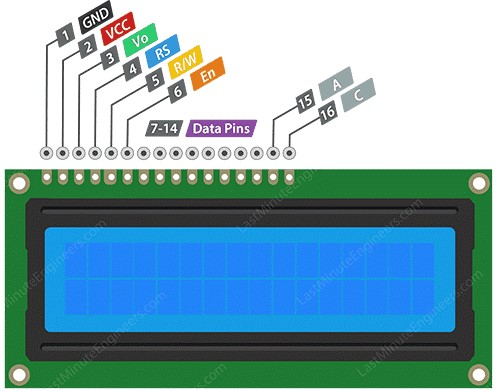
\includegraphics[width=\textwidth]{\LocLDRfig/lcdpinout.jpg}
    \label{fig:pinlcd} \hfill
  \caption{Pinout of 16x2 LCD}
\end{figure} 

\begin{itemize}
  \item \textbf{GND} should be connected to the ground of Arduino.
  \item \textbf{VCC} is the power supply for the LCD which we connect the 5 volts pin on the Arduino
  \item \textbf{Vo (LCD Contrast) } controls the contrast and brightness of the LCD. Using a simple voltage divider with a potentiometer, we can make fine adjustments to the contrast.
  \item \textbf{RS (Register Select) }  pin lets the Arduino tell the LCD whether it is sending commands or the data. Basically, this pin is used to differentiate commands from the data.
For example, when RS pin is set to LOW, then we are sending commands to the LCD (like set the cursor to a specific location, clear the display, scroll the display to the right and so on). And when RS pin is set on HIGH we are sending data/characters to the LCD.
  \item \textbf{R/W (Read/Write) } pin on the LCD is to control whether or not you’re reading data from the LCD or writing data to the LCD. Since we’re just using this LCD as an OUTPUT device, we’re going to tie this pin LOW. This forces it into the WRITE mode.
  \item \textbf{E (Enable) } pin is used to enable the display. Meaning, when this pin is set to LOW, the LCD does not care what is happening with R/W, RS, and the data bus lines; when this pin is set to HIGH, the LCD is processing the incoming data.
  \item \textbf{D0-D7 (Data bus) } are the pins that carries the 8 bit data we send to the display. For example, if we want to see the uppercase ‘A’ character on the display we will set these pins to 0100 0001(according to the ASCII table) to the LCD.
  \item \textbf{A-K (Anode \& Cathode) } pins are used to control the backlight of the LCD.
\end{itemize}


\section{Interfacing the PIR \& LCD through the Arduino IDE}
\label{sec:pir-arduino-code}
\subsection{Interfacing the PIR \& LCD}
Controlling LCD is a quite complicated task. Fortunately, thanks to the LiquidCrystal library, this library simplifies the process of controlling LCD for you so we don't need to know the low-level instructions. We just need to connect Arduino to LCD and use the functions of the library.

\begin{enumerate}
  \item Include the library: 
        \lstinputlisting[firstline=1,lastline=1]
        {\LocLDRardcode/pir-lcd/pir-lcd.ino}
\item Creates an LCD object with parameters: (rs, enable, d4, d5, d6, d7)
        \lstinputlisting[firstline=4,lastline=4]
        {\LocLDRardcode/pir-lcd/pir-lcd.ino}
\item Set up the LCD's number of columns and rows and clear the lcd screen.
        \lstinputlisting[firstline=12,lastline=15]
        {\LocLDRardcode/pir-lcd/pir-lcd.ino}
\item 4.	The cursor is moved to the desired position, and the output “No motion”, “Motion detected!” and “Motion ended” are displayed on the LCD.
        \lstinputlisting[firstline=20,lastline=39]
        {\LocLDRardcode/pir-lcd/pir-lcd.ino}
 

\end{enumerate}


\subsection{Arduino Code}
\label{sec:ldr-arduino-code}
\addtocontents{ard}{\protect\addvspace{\codclr}}

\begin{ardcode}
  \acaption{Read and display the PIR values}
  {Read and display the PIR values.  Available at
    \LocLDRardbrief{ldr-read/led-read.ino}.}
  \label{ard:ldr-read}
  \lstinputlisting{\LocLDRardcode/pir-lcd/pir-lcd.ino}
\end{ardcode}





\section{Interfacing the PIR \& LCD through Python}
\subsection{Interfacing the PIR \& LCD}
In this section, we discuss how to carry out the experiments of the section 2.3.4 from Python. We will list the same experiment. The LCD should be attached to the Arduino Uno board before doing these experiments and the Arduino Uno needs to be connected to the computer with a HC-SR501 PIR Sensor USB cable, as shown in Fig.. The Firmware code given in appendix should be uploaded to the Arduino board.

\begin{enumerate}
  \item  Declare the pin used for the HC-SR501 using a variable and creating a counter variable pirstate and 3 variable nomot, motdet and motend for being used in the function from Step 2.
        \lstinputlisting[firstline=24,lastline=28]
        {\LocLDRpycode/pir-lcd.py} 
 \item The python-based command to print the “Motion detected!”, “Motion ended!” and “No Motion!” are given below respectively.
        \lstinputlisting[firstline=4,lastline=4]
	{\LocLDRpycode/pir-lcd.py} 
 \item Set up the LCD's number of columns and rows and clear the lcd screen.
        \lstinputlisting[firstline=33,lastline=33]
	{\LocLDRpycode/pir-lcd.py}
	\lstinputlisting[firstline=37,lastline=37]
	{\LocLDRpycode/pir-lcd.py}
	\lstinputlisting[firstline=41,lastline=41]
        {\LocLDRpycode/pir-lcd.py} 

\end{enumerate}



\subsection{Python Code}
\label{sec:ldr-python-code}
\addtocontents{pyd}{\protect\addvspace{\codclr}}

\begin{pycode}
  \pcaption{Read and display the LDR values}
  {Read and display the LDR values.  Available at
    \LocLDRpybrief{ldr-read.py}.}
  \label{py:ldr-read}
  \lstinputlisting{\LocLDRpycode/pir-lcd.py}
\end{pycode}

\section{Setup \& Output}
\begin{figure}[hpt]
  \centering
    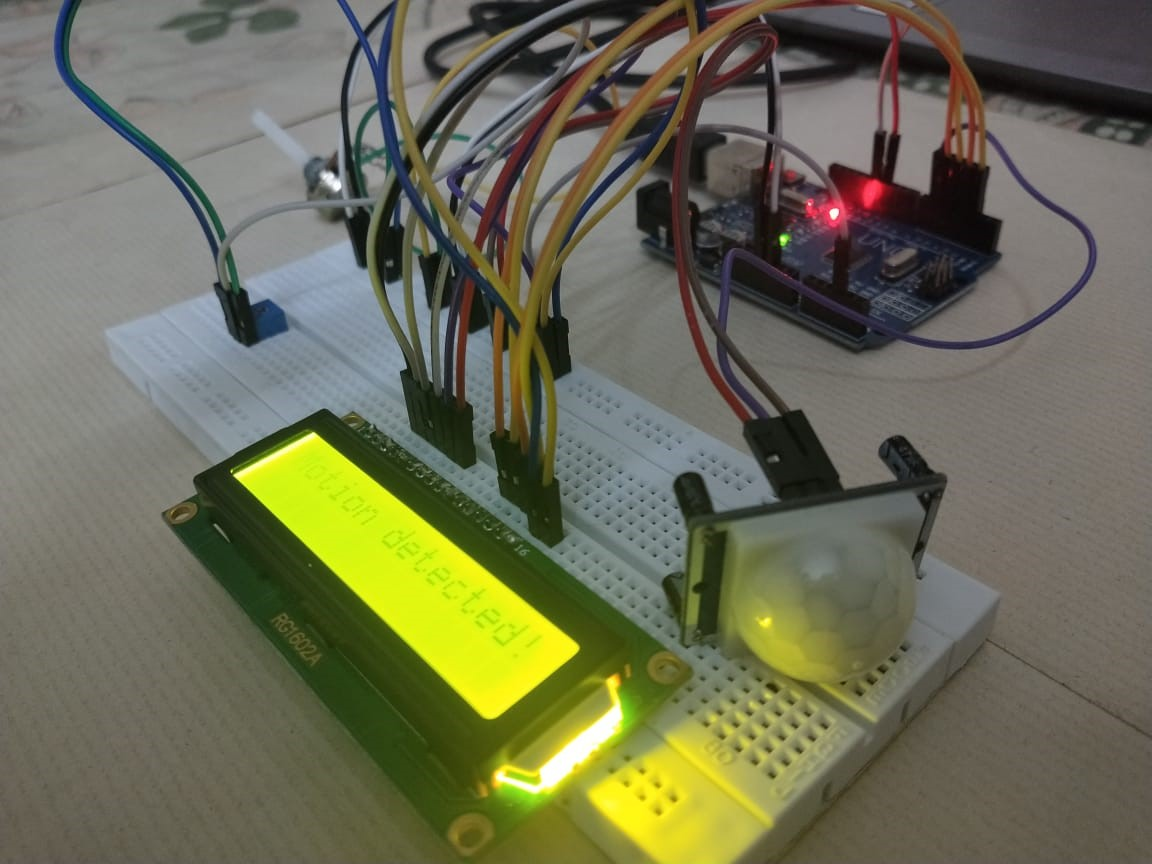
\includegraphics[width=\textwidth]{\LocLDRfig/setup1.jpg}
    \label{fig:set1} \hfill
  \caption{Setup 1}
\end{figure}
\begin{figure}[hpt]
  \centering
    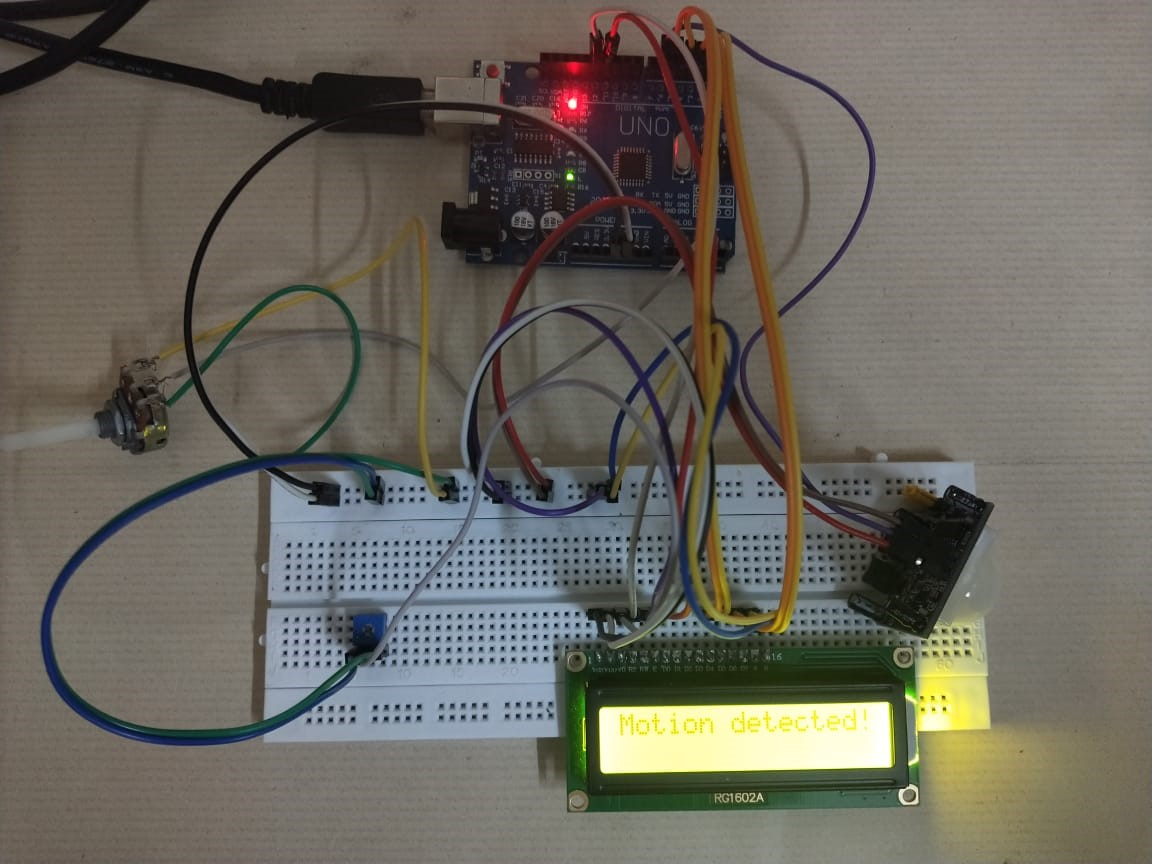
\includegraphics[width=\textwidth]{\LocLDRfig/setup2.jpg}
    \label{fig:set2} \hfill
  \caption{Setup 2}
\end{figure}
\begin{figure}[hpt]
  \centering
    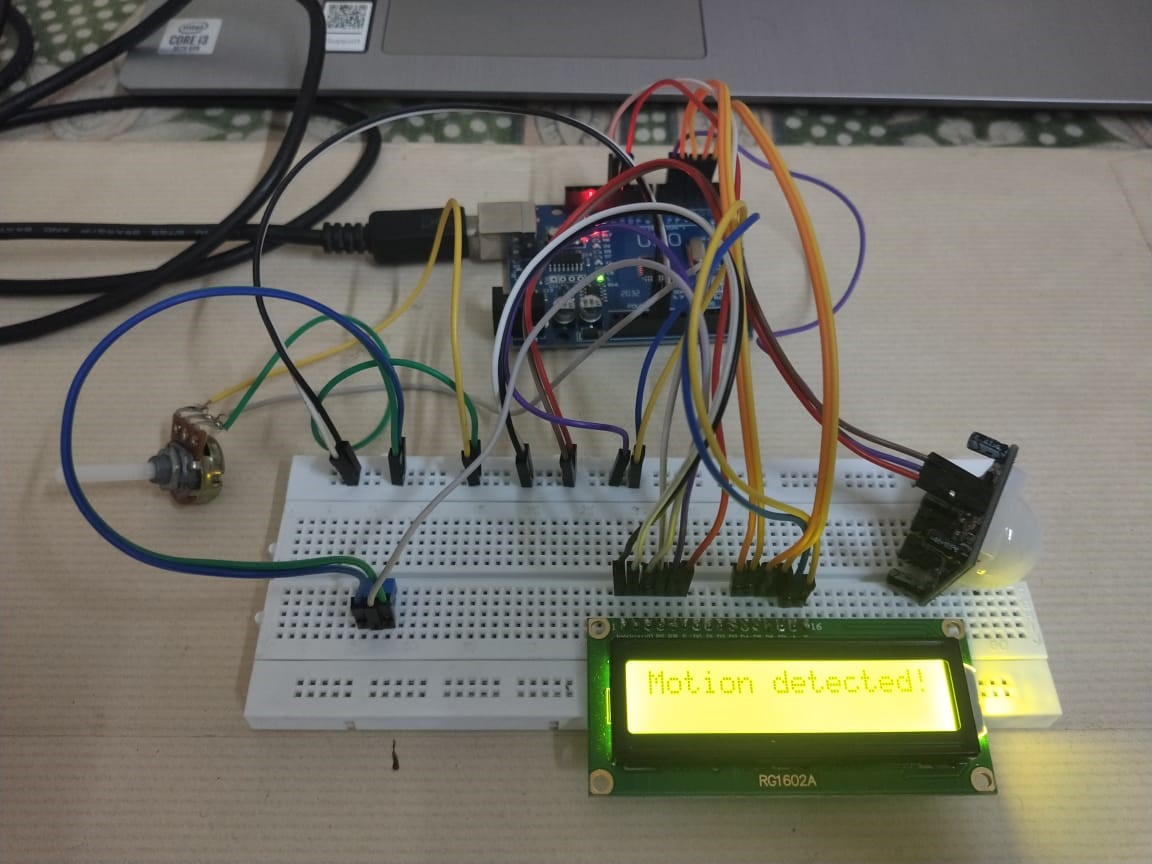
\includegraphics[width=\textwidth]{\LocLDRfig/setup3.jpg}
    \label{fig:set3} \hfill
  \caption{Setup 3}
\end{figure}
\begin{figure}[hpt]
  \centering
    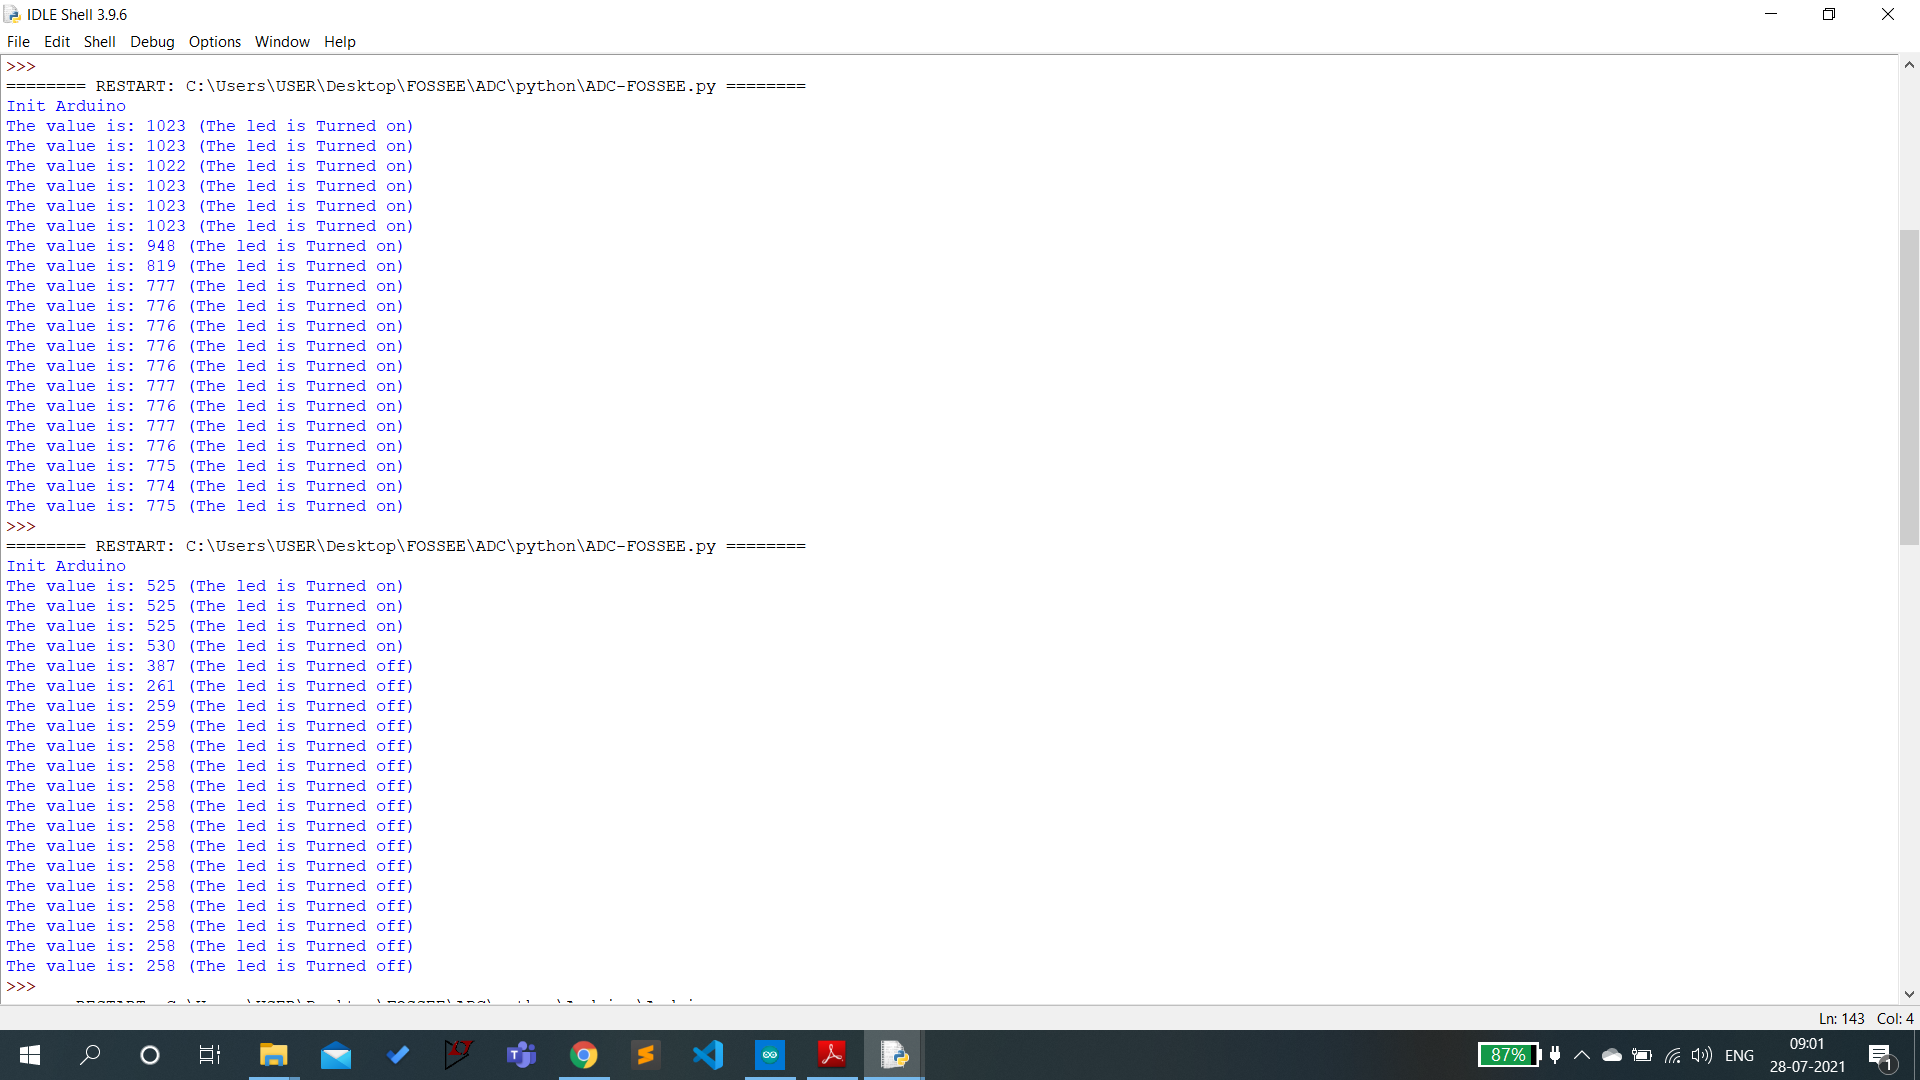
\includegraphics[width=\textwidth]{\LocLDRfig/output1.png}
    \label{fig:out1} \hfill
  \caption{Output 1}
\end{figure}
\begin{figure}[hpt]
  \centering
    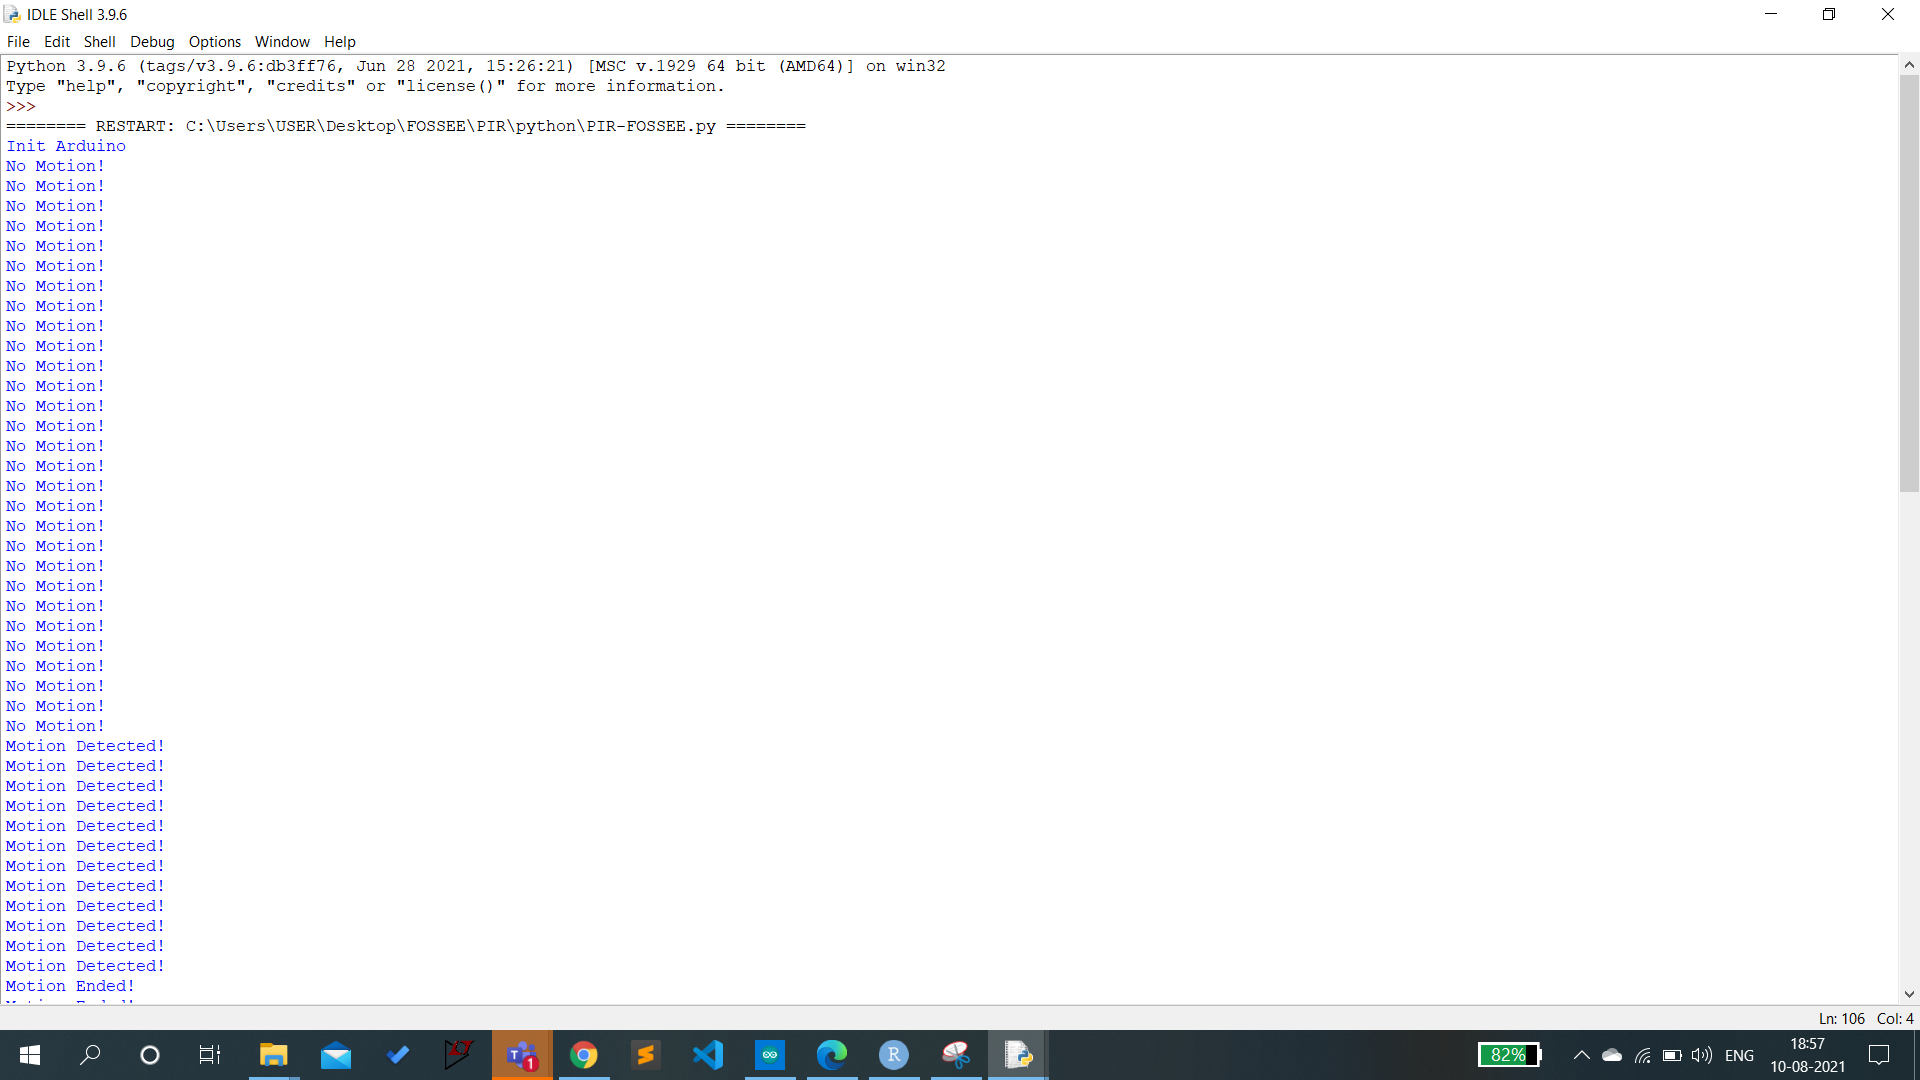
\includegraphics[width=\textwidth]{\LocLDRfig/output2.png}
    \label{fig:out2} \hfill
  \caption{Output 2}
\end{figure}














